\documentclass[12pt]{article}
\usepackage{threeparttable}
\usepackage{rotating}
\usepackage{xcolor}
\usepackage{subfig}


%_ PACKAGES __________________________________________________________________________ %
	
    %__ INPUT/OUTPUT LANGUAGE _________________________________ %
    \usepackage[USenglish]{babel}
    \usepackage[utf8]{inputenc}
    \usepackage[T1]{fontenc}
    %\usepackage{indentfirst}

    %__ MATH __________________________________________________ %
    \usepackage{amsfonts}
    \usepackage{amssymb}
    \usepackage{amsmath}
    \usepackage{amsthm}
    \usepackage{bbm}
    
    %__ THEORY __________________________________________________ %
    \newtheorem{name}{Printed output}
	\newtheorem{lemma}{Lemma}
	\newtheorem{prop}{Proposition}
	\newtheorem{cor}{Corollary}
	\theoremstyle{definition}
	\newtheorem{definition}{Definition}

    %__ GRAPHS & TABLES________________________________________ %
    \usepackage{graphicx}
    \usepackage{subfig}
    \usepackage{booktabs}
    %\usepackage{multirow}
    \usepackage{array}
    \usepackage{caption}
    %\usepackage{subcaption}
    %\usepackage[flushleft,online,para]{threeparttable}
    
    %\usepackage{parskip}                       % WHAT IS THIS FOR?

    \usepackage{floatrow}
        \floatsetup[table]{style=plaintop}     % LEAVE TABLE CAPTIONS AT THE TOP
    %\usepackage[nolists,nomarkers]{endfloat}             % PUT FIGURES AT THE END OF DOCUMENT; DOESN'T WORK WITH \usepackage{float}

    \usepackage{tabularx}
        \newcolumntype{Z}{>{\centering\arraybackslash}X}
        \newcolumntype{L}{>{\raggedright\arraybackslash}X}

    \usepackage{dcolumn}
        \newcolumntype{d}[1]{D{.}{.}{#1}}

    \usepackage{rotating}                      % for **sideways**tables
    \usepackage{lscape}
    \usepackage{pdflscape}

    %__ BIBLIOGRAPHY __________________________________________ %
    \usepackage[round]{natbib}

    %__ PDF, DISPLAY & PRODUCTIVITY ___________________________ %
    \usepackage{xcolor}
        \definecolor{darkblue}{rgb}{0,0,0.4}
    \usepackage{hyperref}
        \hypersetup{
            colorlinks = true,
            linkcolor = darkblue,
            citecolor = darkblue,
            pdfborder = 0 0 0,
            pdfdisplaydoctitle = true,
            pdfhighlight = /N,
            pdfpagelayout = OneColumn,
            pdfpagemode = UseNone,
            pdfstartview = {FitH},
            pdfauthor = {{AB, CF \& JR}},
            pdftitle = {{DYN}},
            pdfsubject = {{}}
        }

    \usepackage[textsize=footnotesize, colorinlistoftodos, textwidth=4cm, obeyDraft]{todonotes}
    %\usepackage{fixme}
        % commands \fxnote; \fxwarnin; \fxerror; \fxfatal
        % \fxsomething{options}{note}{TEXT}* highlights the TEXT

    \usepackage{geometry}
        \geometry{verbose,tmargin=2.5cm,bmargin=2.5cm,lmargin=2.5cm,rmargin=2.5cm}
    \usepackage{setspace}
        \onehalfspacing

    \usepackage[bottom, multiple]{footmisc}    % keep footnotes at the bottom of the page, and allow for multiple footnotes at one place.

    \usepackage{verbatim}
    \usepackage[normalem]{ulem}     % strikethrough fonts
    \usepackage{mathpazo}

    %\usepackage{syntonly}       % if uncommented, this will prevent latex to produce
    %    \syntaxonly             %   any output. latex will only check for syntax.
    %\usepackage[displaymath,tightpage]{preview}
    %\graphicspath{{//graphs/}}

    %__ APPENDIX _____________________________________________ %
    \usepackage[toc,page]{appendix}

%__ COMMANDS _________________________________________________________________________ %
    \newcommand{\mc}{\multicolumn}
    \newcommand{\lbar}{\underline}
    \newcommand{\ubar}{\overline}




\title{\textbf{Can Monitoring and Citations Make Food Safer?}}

\author{Jason Huang}

\date{\bigskip \today}

% _ DOCUMENT _________________________________________________________________________ %

\begin{document}

\newcommand{\cfbox}[2]{%
    \colorlet{currentcolor}{.}%
    {\color{#1}%
    \fbox{\color{currentcolor}#2}}%
}

\maketitle

\begin{abstract}

I estimate the impact of food inspections on restaurant cleanliness by estimating how citations of health code violations affect subsequent inspection results and 311 complaint calls. To address the endogeneity of the inspection outcomes, which conflate detection of the inspectors and the compliance by the restaurants, I exploit the random assignments of inspectors and construct inspector-specific measures of stringency as an instrumental variable. I find that this variable is highly predictive of not only the total scores but also the specific violations that are cited, despite the random assignment process that results in similar restaurant characteristics across inspectors. I find that, on the margin, more citations leads to better subsequent inspection outcomes, and the effects are larger for chain affiliates. I also find that the establishments respond to the most in areas in which they received citations. Furthermore, I document how citations in one area affect results in other areas during subsequent inspections, and these cross-area estimates shed light into the production function of the retail food industry. Lastly, I find that consumers respond to these improved sanitation conditions by making 311 complaint calls less frequently. 

\textit{JEL: D02, D81, D82, K32, L51}\\
\end{abstract}
\thispagestyle{empty} \newpage

\onehalfspacing \setcounter{page}{1}

\section{Introduction}

Food hygiene at restaurants is a great public health concern. The CDC estimates that over 3 million food-borne illnesses occur in the US annually, with 60\% of the cases resulting from dining in restaurants.\footnote{Surveillance for Food borne Disease Outbreaks United States: 2013 Annual Report. Available: https://www.cdc.gov/foodsafety/pdfs/foodborne-disease-outbreaks-annual-report-2013-508c.pdf} Unlike food quality or service, which consumers can observe, food sanitation qualities remain opaque to consumers. Diners usually cannot venture back to the kitchens and monitor the food preparation process. Also they may not have the training or the equipments, such as a thermometer, to spot improper hygiene practices. Local health departments conduct regular food inspections with trained public servants to ensure that restaurants meet certain hygiene standards. Understanding whether these inspections incentivize restaurants to improve their sanitation practices can have important policy implications.

This paper estimates the causal impact of New York City's food inspection results on restaurant compliances and customer perceptions, measured by frequencies of 311 complaints calls. Inspection results can potentially influence restaurant behaviors for two reasons. First reason is monetary. Starting from July 2010, the  New York City's Department of Health and Mental Hygiene (DOHMH) has required restaurants to post letter grades that reflect inspection outcomes on their entrance windows. These grades can influence consumer demand and affect revenues. The second one is behavior. Restaurants may improve by learning from previous mistakes pointed out by the citations. Restaurants may commit violations not because they are profit maximizing by cutting enough corners to equate the marginal savings with the expected marginal cost of penalties. Instead, restaurants may make mistakes because of lack of knowledge or experience.\footnote{Each violation is associated with a fine, and the amount of fine depends on the severity cited by the inspector. However, the amounts of these fines are very small, ranging from 200 to 1000 per violation.} Given that cleanliness is a multi-dimensional task, I also examine how the distribution of citations impact the distributions of efforts across these dimensions. In other words, In addition, I test whether consumers behaviors respond to changes in restaurant hygiene efforts by measuring the changes in the frequencies of 311 complaint calls. The inspection results may affect consumer behaviors through two channels. In the first channel, worse results incentivize restaurants to make substantive improvements, which lead to decreases in calls. In the second channel, worse results lead to lower grades, causing consumers to view the establishment more negatively and more likely to complain. 

I find that more citations lead to improved outcomes during subsequent inspection results. Receiving an one standard deviation worse overall sanitation score leads to an 0.23 standard deviation improvement in the overall score, a 9 percent increase in probability of earning an A, and 62 percent decrease in probability of being temporarily shutdown for unresolved critical violations. While most of the improvement that a citation caused the restaurant to make is in the same area, citations in some areas led to improvements in other areas. For example, I find that an additional citation in Facility Design led to 0.195 fewer citations in Food Protection, in addition to 0.2 fewer citation in Facility Design. After merging the inspection data with the 311 complaint call data, I find evidence that more citations also leads to fewer complain calls, suggesting that customers also notice the improved sanitation qualities. 

I also investigate whether the treatment effects differ across observable characteristics, such as whether an establishment has chain affiliation or the number of reviews and stars on Yelp, a popular crowd-source review site. After combining the inspection data with the restaurants' Yelp information, I find that the restaurants' responsiveness to citations do not depend much on their star ratings or average number of reviews per day. On the other hand, the treatment effects of inspections results for chain restaurants are much larger than those of independent restaurants. For chain restaurants, their subsequent scores respond one third more than and their probabilities of earning As responded more than twice as much as those of independent restaurants. One potential explanation for this heterogeneous treatment effect is that chain restaurants have more standardized menus and kitchen technology, which allow them to promptly correct any hygiene problems. But the fact that the effect on getting As is much larger than the effect on the underlying scores or getting temporarily closed, two outcomes that are much less visible to the general public than the letter grades also suggests that chain restaurants are concerned about the negative repetitional externality that signals of poor hygiene quality can impose on the rest of the brand. 

Even though understanding how small businesses respond to government monitoring and citations should be of interest to academics and policy makers, there is a dearth of studies on this topic. A major empirical challenge is that the variable of interest is endogenous. The inspection results depend on both the effects of monitoring and compliance, and we need to disentangle the two to estimate the causal effect of citations. For example, suppose we find that restaurants that have high numbers of citations tend to have high number of citations in the future. Do more citations lead to worse compliance or do restaurants that did poorly in the past tend to do poorly in future? This paper uses the random assignment of food inspectors to inspections as an instrumental variable to overcome the endogeneity of inspection results. The intuition behind this identification strategy is that, given that different inspectors have different levels of stringencies, the results that restaurants receive are partly determined by chance.\footnote{Other research areas that have used this random assignments of decision makers to recover causal impacts include the impact of incarceration on recidivism \citep{bhuller_16}, the effect of disability insurance on labor supply \citep{Maestas_13}, and the impact of foster care system on child outcomes \citep{Doyle_07}.}

A growing literature that complements this paper focuses on the role of transparency to improve food sanitation and reduce food-borne illnesses. The first type is certification, or what \cite{Ho_2012} calls targeted transparency. Letter grade system, first introduced in Los Angeles, is one example of certification. \cite{jie_leslie_05} and \cite{Simon_05} study the introduction of Los Angeles's grading system in 1998 and find strong evidence for a decrease in hospitalization for food-borne illnesses in jurisdictions after the enactments of the grading systems. \cite{Wong_at_el_2015} and \cite{Meltzer_2015} study New York City's letter grade system. After finding that improved sanitation scores and lower violation fines followed the introduction of the letter grades, they conclude that the reform improved sanitation practices. \cite{Filion_Powell_09} document the growing popularities of these grading programs across the globe. While these papers looks at the impact of the overall inspection programs, I study the effect of individual inspections. The second type of transparency arise from customer reviews. \cite{Luca_13} use Yelp reviews to predict health code violations, and they argue that inspection selection can be optimized based on information from social media. However, sending food inspectors to restaurants for inspections remains as the most direct tool of enforcement, and understanding the impact of these inspections on compliance remains important. Hence, I see this study about monitoring and detection as a complement to instead of a substitute of studies on the role product transparency plays in maintaining food hygiene.

This paper also relates to a broad literature that studies the connection between government monitoring and compliance. Researchers have explored this issue in other areas such as taxation (\cite{Feinstein_91}, \cite{Kleven_etal_10}, \cite{Gemmell_Ratto_12}), workplace safety \citep{levine_etal_12}, nuclear power plants \citep{Feinstein_89}, and environmental protection \citep{Duflo_Greenstone_14}. While \cite{Jin_Lee_12} and \cite{Jin_Lee_14} also examines the food inspection programs, the two papers focus on the inspectors' behaviors and detection technology. \cite{Jin_Lee_14} provide suggestive evidence that improved detection technology lowers the probability of food borne disease outbreaks, it does not provide evidence that links inspector behaviors with restaurant compliance, which this paper does.

The rest of the paper proceed as follows. Section \ref{background} describe the New York City's food inspection program. Section \ref{data} describes the food inspection, Yelp, and 311 data. Section \ref{IV} explains the construction of the instrumental variable and describes various validity tests. Section \ref{empirical_sec} presents the main empirical strategy and discusses the results. Section \ref{conclude} concludes.
\section{New York City Food Inspection and Grading System}
\label{background}

New York City's DOHMH oversees the city's food safety program. It sends out food inspectors to restaurants to conduct inspections, and each restaurant receives at least one inspection a year. Starting in 2005, the city implemented a numerical scoring system, which still exists today. It outlined ninety-eight violations, broken into eight categories: food temperature, food source (general and critical), food protection, facility design, personal hygiene, vermin/garbage, and facility maintenance. Each violation is associated with a range of scores, and the inspector assigns the numerical value that reflects the severity of the violation. For example, a violation 10F for non-food contact surface improperly constructed is worth from 2 to 5 points, with higher scores corresponding to more of these surfaces the inspector finds.\footnote{For more details of how violations are scored, see Food Service Establishment Inspection Procedures Handbook: 

http://www1.nyc.gov/assets/doh/downloads/pdf/about/healthcode/health-code-chapter23.pdf. } On average, an an inspection takes one hour and forty-five minutes. During the inspection, the inspector carries a hand-held computer that records the violations and scores manually inputted by the inspector. 

Starting in 2010, the sum of the scores were converted to letter grades, A, B, C, based on the following cutoffs. Score between 0 to 13 earns an A, between 14 to 27 earns a B, and 28 or above earns a C. In addition, the city required the restaurants to post these letter grades on the entrances so that the letters are clearly visible to the customers. The grading policy also changed the inspection cycles. It introduced dual inspection cycles, which involved the a random initial inspection and a possible re-inspection within a month if the initial inspection results in a letter grade lower than an A. During the time in between the initial inspection and re-inspection, restaurants can either post their assigned letter grade or a sign saying "Grade Pending." The score from re-inspection is then used to determine the letter grade the restaurant posts until the next initial inspection, and the previous initial inspection result has no effect. Inspectors to both cycles are randomly assigned so rarely does the same inspector inspect a restaurant twice in a row. Finally, the time between an initial inspection and the subsequent initial inspection depends on the inspection results from the original inspection. If the initial inspection score is lower than 14, the subsequent inspection occurs in roughly a year. If the score is between 14 and 27, the median time until the next inspection is 201 days. If the score is greater than 27, the median length until the next inspection is 176 days. 

DOHMH may temporarily close a restaurant following an inspection for two reasons. The first reason is that the establishment poses a public health hazard that cannot be addressed by the end of the inspections. Examples of such hazards include hot food not cooked to high enough temperature or cold food not stored at low enough temperature, presence of unpasteurized milk, or harmful noxious gas detected. The second reason is that the restaurants receive scores above 28 for three consecutive inspections. If closed, DOHMH immediately posts a closure sign on the window. To reopen, the establishment must submit a written statement to DOHMH that describes the steps it has taken to correct the violations. Then re-opening inspection occurs. The establishment can re-open if it passes the re-opening inspection, but it receives its next initial inspection within three months. The median time between closure and re-opening inspection is 4 days, with 95\% of the cases occurring within 24 days. Repeat violations may prompt DOHMH to shutdown an establishment for longer or permanently. 

The inspections are conducted by health inspectors with the proper title of Public Health Sanitarians. To qualify, the employee must have either a baccalaureate degree from an accredited college or university, with thirty semester credits in the physical and/or biological sciences, or associate degree from an accredited college or university, with fifteen semester credits in the physical and/or biological science and five years of work experience and completion of public health training course approved by New York State Health Department. As of May 2016, the position offers annual salary of \$42,000.\footnote{\emph{Notice of Examination}: http://www.nyc.gov/html/dcas/downloads/pdf/noes/201606036000.pdf}

\section{Data}
\label{data}
\subsection{Food Inspection Data}

The main data source is the universe of food inspections conducted by New York City's Department of Health and Mental Hygiene (DOHMH) from July 2007 to September of 2016. Each observation in the data corresponds to a violation cited during each inspection. It has information on the date of the inspection, the type of inspection (either initial inspection or re-inspection), anonymized ID of the inspector, the total score from all the violations, date of adjudication if it occurred, and the modified score after adjudication. It also has the name, street address, zipcode, cuisine type, service type, and venue type of the establishment. 

This study focuses on the inspections conducted after the enactment of the grading system, which occurred on July 2010. While sources say the implementation was swift, I use all inspections that occurred after October 1st of 2010 to give 3 month buffer to account potential lags.\footnote{\cite{Ho_2012} says that the actual law was enforced on July 15, 2010.} In the period following the grading system, I see over 337,000 inspections, which include both initial inspections and re-inspections, across over 44,000 establishments inspected by 414 inspectors. 

The Figure \ref{pipeline} shows the distributions of inspection types across the inspection types. We see that over 60\% of initial inspections earn scores higher than 13, resulting in re-inspections. Of the re-inspections, 14.2\% earn Cs, 37.7\% earn Bs, and the remaining earn As. Almost 90\% of re-inspections that do not earn As go to adjudication, with a bit over half getting modified scores that result in improved grades and over 80\% resulting in lower modified scores. 

Table \ref{sum_stat} presents summary statistics for both the restaurant samples and inspection samples. For the restaurant sample, each observation represents a restaurant, and for the inspection sample , each  observation represents an inspection. By comparing the two samples, we can see whether inspections tend to skew towards certain types of restaurants. The statistics appear fairly comparable across the two samples, with restaurants that have counter service being inspected more often and those with takeout service inspected less often. 

\subsubsection{Descriptive Analysis: Bunching Around Thresholds}

As documented in other economic literatures, the discontinuous mapping from integral scores to discrete letter grades creates jumps in incentives and leads to bunching in the score distributions.\footnote{See \cite{Gourio_Roys_14} for discontinuity of firm sizes caused by size-based regulations.} More specifically, as shown in the left plot of figure \ref{bunching}, the distribution of scores from initial inspections clearly show bunching around the cutoff between an A and a B at 13. We do not see any bunching above 13 since all those inspections re-inspections follow and those scores do not contribute to the final  and those restaurants often opt to post Grade Pending in the meantime. In the right plot in figure \ref{bunching}, we see bunching around both 13 and 27 in the scores from re-inspections since those scores contribute to the determination of the letter grades. 

Strategic behaviors of both the inspectors and the restaurants can contribute to the observed bunching in the score distribution. Even though the inspector records the violations in a handheld computer to ensure consistency and accuracy, a claim supported by \cite{Jin_Lee_14}, the inspector can wait until after summing up the scores and adjust what one enters so that the total score does not exceed thirteen. Some potential reasons for inspectors to bunch during the first inspection include saving extra trips for re-inspections or the administrative costs of adjudications.  But given that the same inspector does not inspect conduct the re-inspection, and the adjudication is handled by another department, this explanation is unlikely. The bunching may be driven by restaurant behaviors. The inspection worksheet is publicly available, so the restaurants may that are around the threshold between grades may exert extra effort to improve. A final reason, which is a behavioral explanation, may be that inspectors experience awkwardness handing out a score that is a point or two what is needed to earn a better grade. 

\subsection{311 Calls}

New York's 311 phone lines provide access to non-emergency municipal services, such as fixing potholes or removing dead animals. Another use of the 311 number is for people to call in about food safety or poisoning complaints. The data contain the date of the call, the types of complaints, and the address of the incident. The type of complaint may be one of "Rodents/Insects/Garbage", "Bare Hands in Contact w/ Food", "Food Contains Foreign Object", or "Food Spoiled". I excluded complaints labeled "Letter Grade," which refers to when customers find that letter grades are not shown or not properly placed, as these complaints do not reflect sanitation qualities. The data is provided through NYC's Open Data portal.\footnote{The data portal can be found here: https://nycopendata.socrata.com/Social-Services/311-Service-Requests-from-2010-to-Present/erm2-nwe9} I focused on calls made to DOHMH from 2010 until the 2017, which included 55,476 calls.  

The 311 calls are matched to the food inspection data based on the address using fuzzy string matching. To not bias the analysis against restaurants with no address or address that are difficult to match, I exclude all establishments that share the same address with at least another establishment. This process excludes many concession stands or fast food establishments in major hubs like JFK airport or Grand Central Station. This leaves me with a sample of 40,531 establishments that had at least one inspection after October 2010. The average number of complaint calls between initial inspections is 0.14. The appendix provide more detail on the matching process. 

\subsection{Yelp Data}

Yelp.com is a crowd-sourcing website in which customers write reviews and give a rating on a 5 star scale. A user of Yelp must have a free account to write reviews but a user does not need to register to read others' reviews. The website has an open API that take names and address of a restaurant and returns a json object that includes various Yelp characteristics of the establishment, including the rating score and the number of reviews up to the date of the API call. The open API does not return historical reviews. Instead, it provides only the rating information at the time of the API call. Hence, the data on the star ratings and the numbers of reviews I use in paper are those of the restaurants as of April of 2017, which is when I made the API calls. 

Out of all the restaurants in the food inspection data, I successfully matched 29,000 establishments, based on name, address, and phone number. Table \ref{yelp_comp} shows the summary statistics of restaurants matched and not matched with the Yelp API. We see that the matched sample tend to have more chains, fewer fast food restaurants and fewer cafeteria. 

\section{Stringencies of Inspectors as Instrumental Variable}
\label{IV}
According to staff of DOHMH, whenever a restaurant requires an inspection, whether for an initial inspection or a re-inspection, a inspector is randomly assigned to inspect that establishment. Inspectors do not specialize in any particular geographies or types of restaurants, so every restaurant at any point in time should be equally likely to receive any of the inspectors. In the next subsections, I discuss how I construct the instrumental variable and show its predictive power on the endogenous variable. 
 
\subsection{Inclusion Restriction}
\label{IV_construct}
The inclusion restriction of a instrumental variable requires it to have high predictive power on the endogenous variable. In this case, we need our inspector stringency to be highly correlated with the scores that the inspector assigns to the restaurants. I calculate the instrumental variable for each inspection by computing the average score that the assigned inspector gives to all the other restaurants that the inspector has inspected for that inspection type (initial or re-inspection). Specifically, I define the instrument between restaurant $i$ and inspector $j$ of inspection type $p$ as
\begin{align*}
    Z_{ijp} = \frac{1}{n_{jp} - I_{ijp}} \left( \sum_{kjtp\neq ijtp}  SCORE_{kjtp}\right)
\end{align*}
where $n_{jp}$ is the total number of type $p$ inspections conducted by inspector $j$, $I_{ijp}$ is the total number of type $p$ inspections inspector $j$ has conducted at restaurant $i$, and $SCORE_{kjtp}$ is the score inspector $j$ gave to restaurant $k$ on date $t$ for an inspection type $p$.

Figure \ref{first_stage_fig} plots the distribution of the inspector average scores. The histogram shows a considerable amount of heterogeneity in terms of inspectors' levels of stringencies.\footnote{See \cite{Feinstein_89}, \cite{Feinstein_91}, and \cite{Macher_11} for additional documentation of inspector heterogeneity pertaining to IRS examiners, nuclear power plant inspectors, FDA regulators, respectively.} Figure \ref{first_stage_fig} also shows the fitted value of locally weighted regression of the inspection scores on the inspectors' leave-out average scores.\footnote{I use a bandwidth of 0.5.} The inspection scores and the inspector average scores follow a monotonic relationship, closely tracing along the 45$^\circ$ line. The plot suggests that being inspected by a more stringent inspector correlates with a higher expected score. 

We set up the first stage of our two-stage least square analysis here. 
\begin{align}
score_{it} = \gamma Z_{it} + \delta_i + \tau_t + \epsilon_{it}
\label{first_stage_eq}
\end{align}
Table \ref{first_stage_reg} shows the first stage result of \eqref{first_stage_eq}. It shows the results of both with and without restaurant fixed effects. We see that the point estimates are around 1, which suggests that an inspection done by an inspector with a 1 point higher average score increases the expected inspection score by 1 point. The estimates are also highly statistically significant, suggesting that the inspector stringency is not a weak instrument. 

\subsection{Assessing the Randomness of Inspector Assignment}

While we cannot directly test for the randomness of the inspectors' assignment process, we can test for some empirical patterns that random assignment implies.  

The first implication of random assignment is that the inspector propensity should not be correlated with observables of restaurants to which one is assigned. Hence, we test whether restaurant observable characteristics have predictive power of the stringency levels of the inspectors assigned to them. If the assignments are random, the covariates should all be small and statistically insignificant. For example, a coffee shop in Brooklyn should have the same chance of getting a strict inspector than a Michelin five star restaurant in Manhattan. Table \ref{cond_ind} shows the regression results of inspection scores and inspector leave-out average score on various restaurant characteristics and lag terms. In the first column, we see that all the covariates are highly statistically significant for the score regression. In the second column, we see that almost all of the covariates that are statistically significant in the score regression are no longer statistical significance and the point estimates are very small. There are few covariates, such as Pizza/Italian cuisine, or whether the establishment offers buffet or cafeteria service, that are statistically significant at 90\% or higher level. However, their point estimates are fractions of those in the score regression. Calculating inspector propensity using only 50 inspections may cause some covariates to be significant by chance. The third column restrict the sample to inspections done by inspectors with at least 650 inspections. We see that the covariates that were significant in the second columns are no longer significant. 

A second implication of the randomness is that the inspections each inspector conduct should not be geographically clustered, and each geographic area should not be inspected by only a few inspectors. To test this claim, I calculate the Herfindahl-Hirschman index (HHI) of the zipcodes of the restaurants each inspector has inspected and the HHI of the inspectors that have inspected each zipcode. The results are presented in figure \ref{zip_herf}. The red dotted lines represent the HHI of zipcodes and inspectors under the perfect random case.\footnote{Because inspections are not uniformly distributed, the baseline is calculated based on the sample distributions of inspectors across zipcodes} The takeaway from the figure is that, while no zipcode or inspector exhibit a perfectly random distribution, the overall HHI across inspectors and zipcodes are quite small, suggesting no evidence that inspectors tend to focus on a small geographic area or that certain zipcodes get inspected by only a handful of inspectors. 

\section{Empirical Analysis}
\label{empirical_sec}

\subsection{Impact of Inspection Scores on Subsequent Inspection Results}

In this subsection, I examine the effects of the inspection results on subsequent initial inspection results. I consider three outcomes of health inspections as the dependent variables: the overall score, whether the restaurant receives an A, and whether that restaurant gets temporally shutdown for a critical violation that it cannot correct by the end of the inspection. While the overall score offers a summary of the number of violations cited and the severities of those violations, the two other variables should also be of interest. Given the bunching of scores around the 13-14 threshold, we should not expect the treatment effect to be constant across different score ranges. In addition, increasing the proportion of initial inspections that result in $A$s can reduce administrative costs for DOHMH by reducing the resources devoted to re-inspections. We should also examine temporary shutdowns since these are associated with critical violations that may pose the biggest threat to public health. 

To measure the effect initial inspection scores on subsequent initial inspection outcomes, I estimate the following equation: 
\begin{align}
        Y_{i,t^{next}} = \beta Score_{it} + \delta_i + \tau_{t} + \tau_{t^{next}} + \varepsilon_{it},
        \label{score}
\end{align}
where $Score_{i,t}$ is the score earned by restaurant $i$ on date $t$, $\delta_i$ and $\tau_t$ are the restaurant and date fixed effects, respectively, and $t^{next}$ is the date of the subsequent initial inspection. The error term $\varepsilon_{it}$ is two-way clustered at the inspector and zipcode levels. The time fixed effects control for temporal changes in inspector composition that affects the average level of stringency among active inspectors across time, which can invalidate the conditional independence assumption of the instrument if overall sanitation qualities change across time. I instrument for the term $Score_{it}$ using equation \eqref{first_stage_eq}.  

%%%%%%%%%%%%%%%%%%%%%%%%%%%%%%%%%%
\iffalse
Table \ref{score_impact} shows the regression results. The first table shows the result using the entire sample. The second and third tables show the results broken down by The first two columns show the results of the OLS regressions, followed by the results from the IV regression. The fact that OLS yields positive coefficients while the IV yields negative coefficients suggest that sanitation qualities persists across time. A point higher in the current initial inspection is associated with 0.13 point higher score in the subsequent initial inspection. However, a point higher inspection score leads to an 0.23 point improvement in the subsequent inspection. 

In the case that the restaurant's initial inspection is above 13 and experiences 
\begin{align}
  Score_{i,t^{next}} = \beta_1 Score_{it} + \beta_2 Score_{it^{re-inspect}}+ \delta_i + \tau_{t} + \tau_{t^{re-inspect}}+ \tau_{t^{next}} + \varepsilon_{it},
  \label{score}
\end{align}
\fi
%%%%%%%%%%%%%%%%%%%%%%%%%

Table \ref{Shutdown_A} reports the results. Given that the standard deviation of scores is 14, the result suggests that one standard deviation increase in inspection scores increases the chance of getting an A during next initial inspection by about 3\%, which is a 8.3\% increase relative to the average 36\%. And a half standard deviation increase in score decreases the chance of getting closed from the mean probability of 1.62\% to only 0.9\%. Finally, note that the OLS estimates have smaller magnitude of the same sign or the opposite sign as the IV estimates. The persistence of a restaurant's hygiene quality can cause a positive correlation between current and subsequent inspection results, and OLS fails to account for this omitted variable and biases the estimates upwards. 

\subsection{Heterogenous Effect Based on Chain Affiliation and Yelp Characteristics }

In the last section, I documented the average marginal effect of additional citations on subsequent inspection results, and in this subsection, I test of heterogeneous effects across different types of restaurants. 

First, I test whether chain restaurants respond more to citations than independent restaurants. We may expect chain affiliates to respond more for various reasons. From a reputational stand point, franchised chain restaurants may respond less as they can free-ride on the reputation of the chain brand while company-owned chains may respond more since poor sanitation at one establishment can impose negative externalities on the whole chain, as documented by \cite{jie_leslie_09}.\footnote{37\% drop in the stock price of Chipotle, a company-owned franchise, in second quarter of 2016 following its E Coli outbreak, is a recent example of such negative externality.} From a food production's stand point, chain restaurants may have more standardized kitchen technology and sanitation practices, and they may correct infractions quicker and less costly. In fact, chain restaurants generally have better health inspection outcomes than independent ones. Among chain restaurants' initial inspections, 58\% receive As, 0.83\% result in temporary shutdowns, and the average inspection score is 14.9, but among independents' initial inspections, 33\% receive As, 1.83\% result in temporary shutdowns, and the average score is 21.9.

Table \ref{hetero_chain} presents the results. I find that subsequent scores and the probability of receiving an A for chain restaurants respond more than those of independent establishments. More specifically,  scores for chains responding 40\% more than those of non-chains, and the effect on the probability of getting an A in the subsequent inspection for chains is more than double that of non-chains. I find no heterogeneous effect on temporary closure; the point estimate of -3.45e-05 is around 3\% of the baseline estimate of 0.00109, so it is neither economically nor statistically significant. 

Second, I test whether restaurants with good ratings or ones that have more reviews respond more to citations since they have reputations to uphold, or whether lower rated establishments react more since they need signals of good hygiene to offset for their lower ratings. I test for these heterogeneous treatment effects across different ratings or numbers of reviews per day, which I call \emph{exposure} by adding interaction terms between the scores and the Yelp characteristics. To do this, I introduce two indicator variables: $1_{\{rating_i \geq 4\}}$ for whether restaurant $i$ has rating of 4 or greater and $1_{\{exposure_i \geq e_{med}\}}$ for whether restaurant's exposure is greater than the sample median of 0.05 reviews per day. To test for heterogeneous effect, I run the following regression: 
\begin{align}
\label{yelp_hetero}
Y_{it^{next}} = \tau_t + \delta_i +  \beta_1 Score_{it} + \beta_2 1_{\{rating_i \geq 4\} } \times Score_{it} +  \beta_3 1_{\{exposure_i \geq e_{med} \}} \times Score_{it} \\
+ \beta_4 1_{\{exposure_i \geq e_{med}\}} \times 1_{\{rating_i \geq 4\}}\times Score_{it} + \varepsilon_{it}. 
\end{align}

The coefficients of interests are $\beta_2$, $\beta_3$, and $\beta_4$, which estimates the incremental impact of inspection scores on subsequent inspection outcomes for restaurants that are above 4 stars, exposure higher than the median exposure rate, and above 4 stars with exposure rate higher than the median, respectively. Table \ref{hetero_yelp} presents the results, showing that almost all the coefficients show economically small and statistically insignificant estimates. The only statistically significant estimate is the interaction term between score, $1_{\{rating_i \geq 4\}}$, and $1_{\{exposure_i \geq e_{med} \}}$. The negative point estimate suggests that, for restaurants with high rating and high number of reviews per day, the probability of getting shutdown decreases more by 24\% in response to harsher inspection results. One major weakness with this analysis that helps to explain these null results is that the open source API provides only a snapshot. What matters for heterogeneous treatment effect may be the rating and the exposure at the time of the inspection, and my method suffers from measurement error of the Yelp characteristics that causes the estimates on the heterogeneous treatment effects to attenuate towards zero.

\subsection{Multi-task}

So far, I have used the total score as an one dimensional summary of the inspection results. However, cleanliness is a multi-dimensional task. Therefore, we should ask how citations in one 

A related theoretical motivation comes from \cite{Holmstrom_Milgrom_91}, which present a principal agent model in which the agent has multiple tasks but only a subset of the tasks are monitored by the principal. Their result is in the form of \emph{teaching to the test}, in which the agent shifts effort away from tasks that are hard to monitor towards tasks that are. \cite{Lu_2012} empirically confirms this hypothesis by showing that caregivers of nursing homes shift effort away from areas that are not publicly graded towards areas that are. I also tests for multi-task hypothesis to see if citations in one area leads to worsening conditions in other areas. 

DOHMH has enumerated 82 violation codes, grouped into eight categories: food temperature, food source, food protection, facility design, personal hygiene, vermin, and facility maintenance. Figure \ref{task_pie} provides a visual breakdown of the frequencies by which these violation groups are cited. I represent the result of an inspection using an eight-dimensional vector. Each element of the vector corresponds to one of the eight violation groups and encodes the number of citations in that group. 

I test how restaurants' effort allocation responds to the citation profile using the following regression: 
\begin{align}
\label{multi_second}
    Pr(Cited_{igt^{next}}) = \sum_{g' \in \mathcal{G}} \beta_{gg'} Cited_{igt} + \delta_i + \tau_t + \tau_{t^{next}} + \varepsilon_{igt},
\end{align}
where $Cited_{igt}$ is an indicator for whether restaurant $i$ receives a citation of violation in group $g$ on date $t$, $\tau_t$ is the date fixed effect on date $t$, and $\delta_i$ is the restaurant fixed effect. The coefficient $\beta_{gg'}$ measures how a restaurant's effort in group $g$ responds to a citation in group $g'$. As before, $Cited$ is an endogenous variable, so I use instrumental variables. To do so, I construct each inspector's average number of citations in group $g$ by using a leave-out strategy similar to the one done in section \ref{IV_construct}. More specifically, I construct the instrument of inspector $j$'s tendency to cite group $g$ at restaurant $i$ as
\begin{align*}
  Z_{ijg} = \frac{1}{n_j - n_{ij}} \left(\sum_{kjgt \neq ijgt} Cited_{ijgt}\right),
\end{align*}
where $n_j$ is the number of inspections made by inspector $j$ and $n_{ij}$ is the number of inspections inspector $i$ has made at restaurant $j$. The first stage is a system of equations defined as
\begin{align}
\label{multi_first}
    Pr(Cited_{ijgt}) = \sum_{g'\in \mathcal{G}} \theta_{gg'}Z_{ijg'} + \varepsilon_{ijgt}, 
\end{align}
where $\mathcal{G}$ is the set of violation groups. The coefficients $\theta_{gg'}$ measures the predictive power of an inspector's tendency to cite a violation in group $g'$ on the citation of a violation in group $g$. We should expect $\theta_{gg}$ for all the groups to be statistically significant, since the expected number of citations in a particular area should increase with the level of stringency an inspector holds for that area.

Table \ref{multi_first_reg} presents the results of the \eqref{multi_first}. As expected, all the $\theta_{gg}$'s are highly statistically significant and almost all are close to 1. Furthermore, most of the off-diagonal coefficients are either positive or negative but statistically insignificant, suggesting that receiving an inspector who is more stringent on one dimension does not decrease the chance of being cited in another dimension. There are some coefficients, boxed in blue, that are negative and statistically significant at the 1\% level. For example, I find that when a restaurant gets an inspector whose expected number of citation for Facility Design is one unit higher, the restaurant's expected number of citations in Food Protection goes down by 0.337. 

Table \ref{multi_second_reg} presents the results of \eqref{multi_second} instrumenting with \eqref{multi_first}. We see that the diagonal coefficients, color coded in blue, are all negative, and six of the eight groups are statistically significant at 90\% level. I find that the area of Facility Maintenance responds the most in response to citations in the same area, with one additional citation leading to a 0.236 fewer expected citations in the subsequent inspection. 

The signs of the off-diagonals offer insights into the production function of restaurant cleanliness. Many off-diagonal elements are negative and statistically significant, color coded in red. A negative estimate suggests that a citation in one dimension leads to an improvement in another dimension. This finding makes sense in light of the fact that various dimensions may be complementary. One example of such complementarity is that a citation in Food Protection also reduces the expected number of citations from subsequent inspections in Facility Maintenance and Vermin/Garbage by -0.0776 and 0.0397, respectively. A citation in Food Protection may lead the restaurant to improve along this dimension, which might include fixing a broken thermometer (violation 10E) that improves the Facility Maintenance dimension or better maintaining contact surface (violation 10F) that makes the kitchen more vermin proof. We also see a few positive and statistically significant off-diagonal estimates, color coded in brown. For example, a citation in the area of vermin/garbage leads to 0.132 more citations in Facility Maintenance. 

\subsection{Impact of Inspection Results on 311 Complaint Calls}
\label{complaints_analysis}
The ultimate goal of any food inspection programs is to reduce food-borne illnesses. But directly studying the impact on food poisoning is difficult. Most food poisoning incidents go unreported. More severe cases that result in hospitalization leave medical records, but we cannot trace the origins of the illnesses back to specific establishments. Health inspection results serve as convenient proxies for restaurant cleanliness. A couple studies have found correlations between inspection results and the likelihoods of food-borne illness outbreaks.\footnote{See \cite{Irwin_89}, \cite{petran_12} and \cite{petran_12_a}.} In this section, I use 311 complaint calls against restaurants as an additional proxy variable for food hygiene to supplement the findings in my previous sections. The advantage of 311 calls over hospitalization records is that we can trace 311 calls back to specific establishments on specific dates.

I transform the inspection level data to a restaurant-month level panel data in which each observation corresponds to a month for a given restaurant. For each observation, I calculate the inspection score as the score from a restaurant's most recent inspection, either initial or re-inspection. For months when inspections occur and scores change in the middle, I count those restaurants to have had complaint calls only if the calls occurred after the date of the inspection and before the end of the months. To estimate the impact of inspection results on the probability that a restaurant receives a complaint call, I run the following regression:
\begin{align}
\label{complaint}
    Pr(called_{it}) = \delta_i + \tau_t + \beta_0 Score_{it} + \beta_1 Month\_Since\_Inspection_{it} \nonumber \\
    + \beta_2 month\_since\_inspection_{it} \times Score_{it} + \varepsilon_{it}
\end{align}
where $called_{it}$ is a binary variable that equals one if DOHMH received at least one complaint call for restaurant $i$ in month $t$, and $month\_since\_inspection_{it}$ is the number of months since restaurant $i$ in month $t$ has had its last inspection, either initial or re-inspection. The coefficient $\beta_2$ estimates the differential impact of inspection score on the probability of complaint call with an additional month that has elapsed since the last inspection, which in effects tests for heterogeneous effect across time. 

Table \ref{calls} presents the results of \eqref{complaint}. We see that getting a one standard deviation worse inspection score lowers the probability of a 311 call in a month by around 0.01\%, which is almost a 7\% reduction relative to the sample average of 1.45\%. The OLS estimate in column (1) is less negative than IV estimate in column (4). This relation agrees with the fact that OLS does not dis-entangle the treatment effect from the selection bias of restaurants during periods of poor sanitation qualities receiving higher inspection scores, which have opposing effects. When including the $month\_since\_inspection$ interaction term, the point estimate of the baseline estimate decreases and its standard error increases. In turn, neither the baseline coefficient nor the interaction term coefficient is statistically significant, suggesting no evidence that the treatment effect changes across time. A caveat to this analysis is that complaint calls are fairly rare events and the IV estimates are not very precise. But we can interpret these results as suggestive evidence that consumers also respond to the improved sanitation qualities following health citations. 

\section{Conclusion}
\label{conclude}
This paper estimates how restaurants' hygiene qualities responds to citations from government conducted food inspections by identifying a causal link between the inspection result of a given day on the inspection result during and complaint calls up to the subsequent inspection. To overcome the problem of omitted variable bias that may correlate with both current and subsequent inspection results and argue a causal story, I use the random assignments of inspectors restaurants and the heterogeneity in inspector stringencies to construct an instrumental variable. 

I find evidence that restaurants hygiene qualities improve in response to health code citations. Receiving a harsher inspection result leads to improved inspection score, higher chance of getting an A, and lower chance of temporary shutdown during the subsequent inspection. 

These cross-group estimates have implications for the design of the grading rubric or the levels of fines associated with various violations.


\newpage

\bibliographystyle{apa}

\bibliography{Biblio}

\newpage

\section{Appendix}

\subsection{Monotonicity}

The instrument needs only the conditional independence and exclusion restriction to recover the causal effect of inspection results if the effect is constant across establishments. With heterogeneous effects, however, we need monotonicity condition. In this setting, the condition states that the score that an establishment gets is strictly increasing in the stringency of the inspector. This is a condition that we cannot directly test since it requires the scores of counterfactual establishments inspected by inspectors of different stringency. This condition can be in question when the treatment depends on multi-dimensions and inspectors differ not only in overall stringency but across those dimensions. For example, suppose that we have a stringent and lenient inspector, but the lenient inspector is much more picky about keeping cold food under the proper temperature than the stringent inspector. Then a sushi restaurant that serves a lot of raw fish can conceivably receive a worse score when it gets the lenient inspector. 

To appease such concern, I follow the strategy used in \cite{bhuller_16} and conduct two tests. First, I test whether the first stage holds for various sub-samples based on overall cleanliness, boroughs, cuisines, and service. The overall cleanliness is calculated as the predicted values from regressing scores on restaurant fixed effect, inspection date fixed effects and inspection type fixed effects. I split the samples into four quartiles based on the predicted values. Second, I reconstruct the inspector stringency by excluding the sub-sample of interest. For example, in the case of inspections done in Manhattan, I recalculate the inspectors' propensities based on the their inspections outside of Manhattan. Monotonicity condition implies that inspectors who are strict for certain establishments are also strict at others. 

Table \ref{mono_test} reports the results for the two tests, organized by cleanliness quartiles, boroughs, cuisine, and service. Each subtable shows the regressions of the original leave-out stringency levels and the re-calculated stringency based on inspections outside of the subsamples. All the estimates are large and statistically significant, suggesting that inspectors' tendencies remain consistent across different types of establishments. 

\begin{table}[!htbp]
\caption{Monotonicity Test}
\label{mono_test}
\subfloat[Cleanliness Quartiles]{\scalebox{0.6}{\begin{tabular}{lcccc}
\multicolumn{5}{c}{Baseline-Sample} \\ \hline
 & (1) & (2) & (3) & (4) \\
VARIABLES & 1st Quartile & 2nd Quartile & 3nd Quartile & 4th Quartile \\ \hline
Estimate & 0.407*** & 0.681*** & 0.852*** & 1.231*** \\
 & (0.0270) & (0.0240) & (0.0213) & (0.0256) \\
 Observations & 80,172 & 81,817 & 81,901 & 86,433 \\ \hline
\multicolumn{5}{c}{ Robust standard errors in parentheses} \\
\multicolumn{5}{c}{ *** p$<$0.01, ** p$<$0.05, * p$<$0.1} \\
\end{tabular}
 \begin{tabular}{lcccc}
\multicolumn{5}{c}{Inverse-Sample} \\ \hline
 & (1) & (2) & (3) & (4) \\
VARIABLES & 1st Quartile & 2nd Quartile & 3nd Quartile & 4th Quartile \\ \hline
Estimate & 0.369*** & 0.612*** & 0.779*** & 1.609*** \\
 & (0.0340) & (0.0247) & (0.0254) & (0.0674) \\
 Observations & 75,188 & 81,328 & 81,481 & 85,851 \\ \hline
\multicolumn{5}{c}{ Robust standard errors in parentheses} \\
\multicolumn{5}{c}{ *** p$<$0.01, ** p$<$0.05, * p$<$0.1} \\
\end{tabular}
 }}

\subfloat[Boroughs]{\scalebox{0.6}{\begin{tabular}{lccccc}
\multicolumn{6}{c}{Baseline-Sample} \\ \hline
 & (1) & (2) & (3) & (4) & (5) \\
VARIABLES & Manhattan & Bronx & Brooklyn & Queens & Staten-Isl \\ \hline
Estimate & 1.005*** & 1.082*** & 0.985*** & 0.969*** & 0.944*** \\
 & (0.0156) & (0.0275) & (0.0198) & (0.0206) & (0.0286) \\
 Observations & 131,900 & 31,010 & 79,664 & 77,186 & 10,507 \\ \hline
\multicolumn{6}{c}{ Robust standard errors in parentheses} \\
\multicolumn{6}{c}{ *** p$<$0.01, ** p$<$0.05, * p$<$0.1} \\
\end{tabular}
 \begin{tabular}{lccccc}
\multicolumn{6}{c}{Inverse-Sample} \\ \hline
 & (1) & (2) & (3) & (4) & (5) \\
VARIABLES & Manhattan & Bronx & Brooklyn & Queens & Staten-Is.\\ \hline
Estimate & 0.990*** & 1.082*** & 0.954*** & 0.934*** & 0.938*** \\
 & (0.0269) & (0.0344) & (0.0238) & (0.0248) & (0.0308) \\
 Observations & 128,977 & 30,334 & 76,973 & 74,933 & 10,468 \\ \hline
\multicolumn{6}{c}{ Robust standard errors in parentheses} \\
\multicolumn{6}{c}{ *** p$<$0.01, ** p$<$0.05, * p$<$0.1} \\
\end{tabular}
 }}

\subfloat[Cuisines]{\scalebox{0.6}{\begin{tabular}{lccccc}
\multicolumn{6}{c}{Baseline-Sample} \\ \hline
 & (1) & (2) & (3) & (4) & (5) \\
VARIABLES & American & Pizza/Italian & Chinese & Coffee & Japanese \\ \hline
Estimate & 0.957*** & 0.994*** & 1.086*** & 0.796*** & 1.096*** \\
 & (0.0241) & (0.0180) & (0.0402) & (0.0354) & (0.0262) \\
 Observations & 75,330 & 38,432 & 38,785 & 13,303 & 10,915 \\ \hline
\multicolumn{6}{c}{ Robust standard errors in parentheses} \\
\multicolumn{6}{c}{ *** p$<$0.01, ** p$<$0.05, * p$<$0.1} \\
\end{tabular}
 \begin{tabular}{lccccc}
\multicolumn{6}{c}{Inverse-Sample} \\ \hline
 & (1) & (2) & (3) & (4) & (5) \\
VARIABLES & American & Pizza/Italian & Chinese & Coffee & Japanese \\ \hline
Estimate & 0.929*** & 0.990*** & 1.070*** & 0.782*** & 1.098*** \\
 & (0.0298) & (0.0199) & (0.0449) & (0.0363) & (0.0273) \\
 Observations & 74,954 & 38,312 & 38,424 & 13,292 & 10,910 \\ \hline
\multicolumn{6}{c}{ Robust standard errors in parentheses} \\
\multicolumn{6}{c}{ *** p$<$0.01, ** p$<$0.05, * p$<$0.1} \\
\end{tabular}
  }}

\subfloat[Service]{\scalebox{0.6}{\begin{tabular}{lccc}
\multicolumn{4}{c}{Baseline-Sample} \\ \hline
 & (1) & (2) & (3) \\
VARIABLES & Counter Service & Takeout Service & Wait Service \\ \hline
Estimate & 1.055*** & 0.894*** & 1.127*** \\
 & (0.0177) & (0.0140) & (0.0178) \\
 Observations & 127,981 & 127,365 & 73,381 \\ \hline
\multicolumn{4}{c}{ Robust standard errors in parentheses} \\
\multicolumn{4}{c}{ *** p$<$0.01, ** p$<$0.05, * p$<$0.1} \\
\end{tabular}
 \begin{tabular}{lccc}
\multicolumn{4}{c}{Inverse-Sample} \\ \hline
 & (1) & (2) & (3) \\
VARIABLES & Counter Service & Takeout Service & Wait Service \\ \hline
Estimate & 1.064*** & 0.810*** & 1.160*** \\
 & (0.0269) & (0.0181) & (0.0236) \\
 Observations & 126,011 & 124,867 & 72,645 \\ \hline
\multicolumn{4}{c}{ Robust standard errors in parentheses} \\
\multicolumn{4}{c}{ *** p$<$0.01, ** p$<$0.05, * p$<$0.1} \\
\end{tabular}
  }}

\footnotetext{The baseline sample regressions use the whole sample to calculate the instrumental variable, while the inverse sample uses all inspection outside of the given sub-sample to calculate the instrumental variable. Standard errors are two-way clustered at inspector and zipcode level. To reduce noise, only inspections conducted by inspectors who have done at least 50 inspections remain in the regressions. }
\end{table}

\subsection{Matching 311 calls to Food Inspection Data}
I use fuzzystring matching to link 311 complaint calls with food inspection data based on the address. I perform following steps to standardize the address:
\begin{itemize}
\item Add suffix to street numbers, i.e. change "1 Street" to "1st Street"
\item Standardize street names, i.e change "Sixth Ave" and "6th Ave" to "Ave of Americas"
\item Manually fix mis-spellings
\end{itemize}

After standardizing the address, I first join based on exact string match. For addresses that do not have exact matches, I consider two a match if they share the same zipcode, the same street number, and if the street names are no further off than normalized Levenshtein distance of 0.1.\footnote{The Levenshtein distance between two strings equals the number of character changes needed to transform one string to another. The normalized Levenshtein distance equals the Levenshtein distance divided by the joint length of the strings in analysis.}

%%%%%%%%%%%%%%%%%%%%%%%%% Data Section %%%%%%%%%%%%%%%%%%%%%%
\newpage

\begin{figure}[!htbp]
\centering
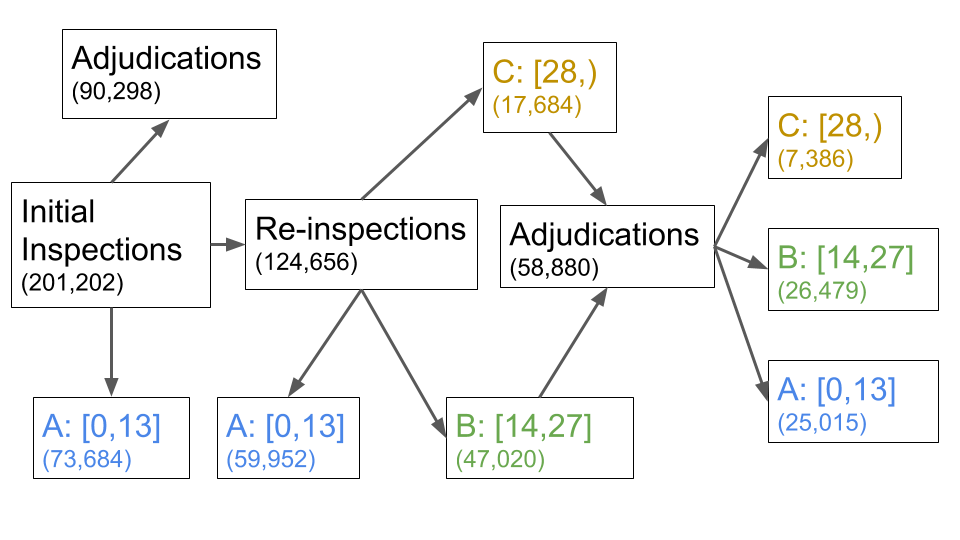
\includegraphics[scale = 0.5]{Figures/Scores.png}
\caption{The Breakdown of Inspections Across the Inspection Cycle.}
\footnotetext{Sample consists of all cycle-inspections after 10/1/2010. In each box, the range in the first line corresponds to the grades, and the number in the second line corresponds to the number of inspections that fall  }
\label{pipeline}
\end{figure}

\newpage

\begin{table}[!htbp]
\centering
\caption{Summary Statistics of Restaurants and Inspections}
\label{sum_stat}
{
\def\sym#1{\ifmmode^{#1}\else\(^{#1}\)\fi}
\begin{tabular}{l*{2}{c}}
\hline\hline
                    &\multicolumn{1}{c}{Restaurant Sample}&\multicolumn{1}{c}{Inspection Sample}\\
                    &        mean&        mean\\
\hline
chain               &       0.112&       0.104\\
Fast Food           &       0.019&       0.016\\
Bar                 &       0.057&       0.061\\
Buffet Service      &       0.015&       0.018\\
Cater Service       &       0.005&       0.004\\
Counter Service     &       0.335&       0.387\\
Take-out Service    &       0.440&       0.386\\
Wait Service        &       0.182&       0.222\\
Cafeteria Service   &       0.010&       0.009\\
\hline\hline
\end{tabular}
}

\footnotetext{This table presents the summary statistics on the sample of inspections after October 1 2010. For the restaurant sample, each observation represents a restaurant, and for the inspection sample , each  observation represents an inspection.}
\end{table}

\begin{table}[!htbp]
\centering
\caption{Summary Statistics of Restaurants Matched and Not Matched Through Yelp API}
\label{yelp_comp}
{
\def\sym#1{\ifmmode^{#1}\else\(^{#1}\)\fi}
\begin{tabular}{l*{2}{c}}
\hline\hline
                    &\multicolumn{1}{c}{Not Matched}&\multicolumn{1}{c}{Matched}\\
                    &        mean&        mean\\
\hline
chain               &       0.080&       0.153\\
Fast Food           &       0.022&       0.016\\
Bar                 &       0.057&       0.056\\
Buffet Service      &       0.015&       0.015\\
Cater Service       &       0.006&       0.003\\
Counter Service     &       0.311&       0.367\\
Take-out Service    &       0.454&       0.423\\
Wait Service        &       0.167&       0.201\\
Cafeteria Service   &       0.014&       0.005\\
\hline\hline
\end{tabular}
}

\footnotetext{This table presents the summary statistics on the restaurants that had at least one inspection after October 1 2010. For both samples, each observation represents a restaurant.}
\end{table}

\newpage 

\begin{figure}[!htbp]
\centering
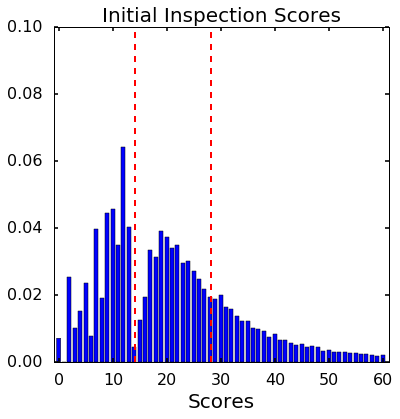
\includegraphics[scale = 0.5]{Figures/init_score.png}
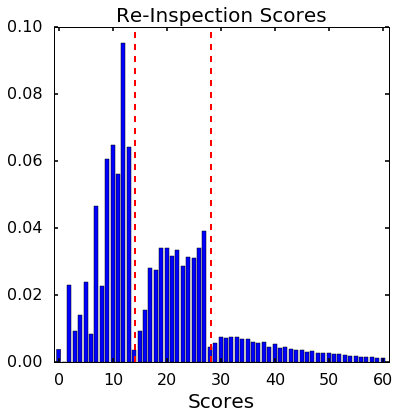
\includegraphics[scale = 0.5]{Figures/re_score.png}
\caption{Score Distribution of Initial Inspections and Re-inspections.}
\label{bunching}
\footnotetext{This figure displays the distribution of inspection scores during initial inspections and re-inspections. The dotted red line represents the 13-14 points and 27-28 thresholds.}
\end{figure}

%%%%%%%%%%%%%%%%%%%%%%%% Inspector Section %%%%%%%%%%%%%%%%%%%%%%%

\begin{figure}[h!]
\centering
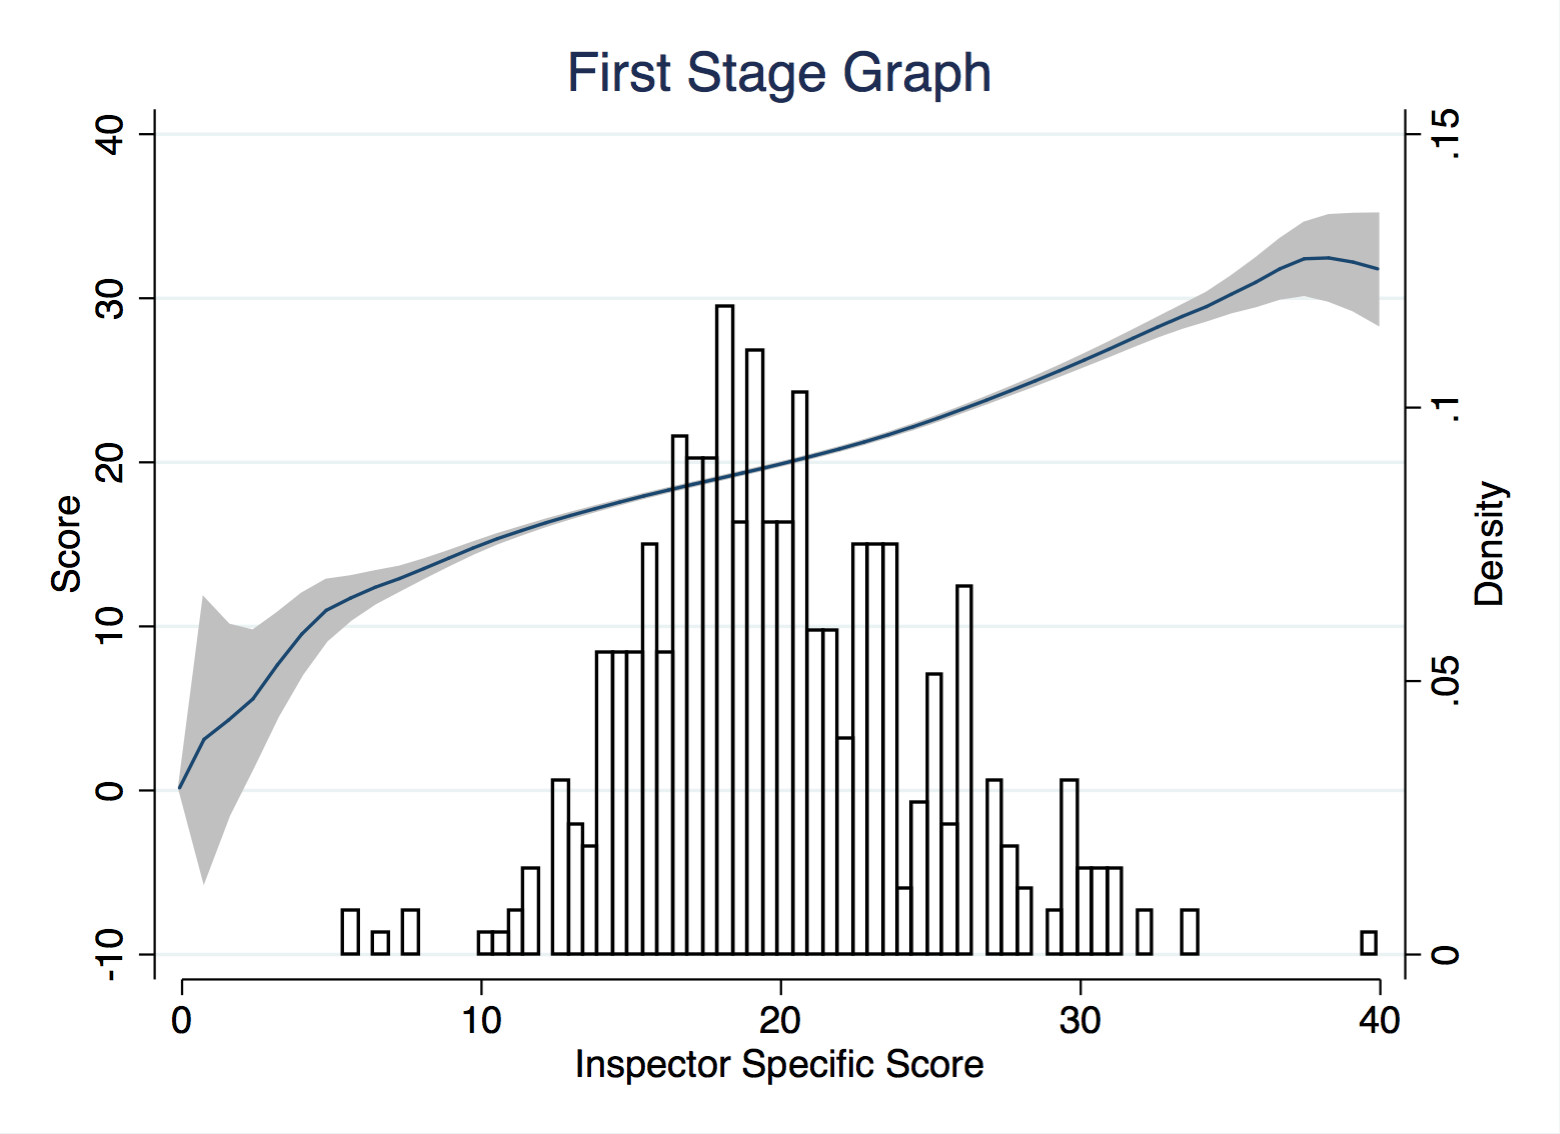
\includegraphics[scale = 0.5]{Figures/first_stage_score.png}
\caption{}
\footnotetext{The plot is generated based on 156,323 initial inspections conducted by inspectors who had done at least 50 initial inspections. The expected inspection score on the left y-axis is plotted against the leave-out average inspector scores on the x-axis. The right axis shows the density of inspector average scores.}
\label{first_stage_fig}
\end{figure}

\newpage

\begin{table}[h!]
\centering
%\subfloat[Full]{\begin{tabular}{lccc} \hline
 & (1) & (2) & (3) \\
VARIABLES & Score & Score & Score \\ \hline
 &  &  &  \\
Z & 0.961*** & 0.997*** & 1.135*** \\
 & (0.00948) & (0.00983) & (0.0162) \\
 &  &  &  \\
Observations & 330,469 & 330,466 & 325,681 \\
R-squared & 0.149 & 0.201 & 0.414 \\
Restaurant Controls & NO & YES & NO \\
Restaurant FE & NO & NO & YES \\
 F Statistics & 10271 & 10270 & 4908 \\ \hline
\multicolumn{4}{c}{ Robust standard errors in parentheses} \\
\multicolumn{4}{c}{ *** p$<$0.01, ** p$<$0.05, * p$<$0.1} \\
\end{tabular}
}

\subfloat[Initial Inspections]{\begin{tabular}{lccc} \hline
 & (1) & (2) & (3) \\
VARIABLES & Score & Score & Score \\ \hline
 &  &  &  \\
Z & 0.945*** & 0.952*** & 0.989*** \\
 & (0.0125) & (0.0131) & (0.0147) \\
 &  &  &  \\
Observations & 200,623 & 200,620 & 192,356 \\
R-squared & 0.141 & 0.208 & 0.475 \\
Restaurant Controls & NO & YES & NO \\
Restaurant FE & NO & NO & YES \\
 F Statistics & 5685 & 5264 & 4537 \\ \hline
\multicolumn{4}{c}{ Robust standard errors in parentheses} \\
\multicolumn{4}{c}{ *** p$<$0.01, ** p$<$0.05, * p$<$0.1} \\
\end{tabular}
}

%\subfloat[Re-inspections]{\begin{tabular}{lccc} \hline
 & (1) & (2) & (3) \\
VARIABLES & Score & Score & Score \\ \hline
 &  &  &  \\
Z & 0.948*** & 0.959*** & 0.997*** \\
 & (0.0111) & (0.0111) & (0.0150) \\
 &  &  &  \\
Observations & 123,226 & 123,220 & 113,385 \\
R-squared & 0.125 & 0.162 & 0.460 \\
Restaurant Controls & NO & YES & NO \\
Restaurant FE & NO & NO & YES \\
 F Statistics & 7320 & 7528 & 4431 \\ \hline
\multicolumn{4}{c}{ Robust standard errors in parentheses} \\
\multicolumn{4}{c}{ *** p$<$0.01, ** p$<$0.05, * p$<$0.1} \\
\end{tabular}
}
\footnotetext{First column consists of all inspections after 10/1/2010. The sample for the second column is reduced to inspections with non-empty zipcode, chain affiliate indicator, cuisine type, venue type, and service type. The Standard errors are two-way clustered at the inspector and zipcode level.}
\caption{First Stage Regression of Inspection Score on Inspector Stringency}
\label{first_stage_reg}
\end{table}

\begin{figure}[h!]
\centering
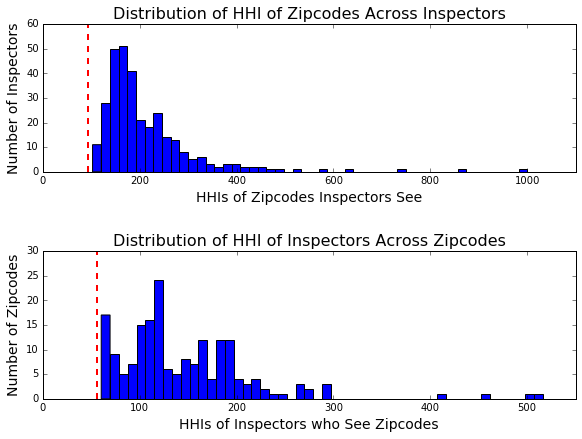
\includegraphics[scale = 0.7]{Figures/zip_herf.png}
\caption{Distribution of HHI}
\footnotetext{The red line represents the expected Herfindahl-Hirschman index of random assignment, with the probability of assigning an inspector being proportional to the number of inspections in that zipcode.}
\label{zip_herf}
\end{figure}

\begin{table}[h!]
\scalebox{0.65}{
\begin{tabular}{lcccccc} \hline
VARIABLES & Score &  & Inspector Stringency &     & Inspector Stringency  &  \\ 
VARIABLES & (> 50 Inspections) & se &  (> 50 Inspections) & se & (> 650 Inspections) & se \\ \hline
last score & 0.218*** & (0.00746) & -0.000440 & (0.00199) & -0.00193 & (0.00205) \\
last grade = B & 1.430*** & (0.131) & 0.0178 & (0.0628) & 0.0837 & (0.0683) \\
last grade = C & 1.495*** & (0.206) & -0.0494 & (0.0764) & 0.0240 & (0.0807) \\
last inspector propensity & -0.298*** & (0.0104) & -0.00363 & (0.00491) & -0.00529 & (0.00551) \\
chain & -3.644*** & (0.179) & -0.0274 & (0.0644) & -0.0300 & (0.0734) \\
Sea Food & 0.301 & (0.412) & -0.0687 & (0.129) & -0.0648 & (0.136) \\
Chinese & 1.588*** & (0.307) & -0.0952* & (0.0510) & -0.0511 & (0.0546) \\
Pizza/Italian & 0.305** & (0.118) & -0.0893*** & (0.0342) & -0.0614 & (0.0384) \\
Coffee/Tea & -2.219*** & (0.162) & -0.0421 & (0.0889) & -0.0514 & (0.0966) \\
Latin & 1.534*** & (0.303) & -0.0714 & (0.0556) & -0.0390 & (0.0583) \\
Spanish & 1.560*** & (0.261) & 0.0125 & (0.0615) & -0.0435 & (0.0691) \\
Caribbean & 1.542*** & (0.288) & -0.0637 & (0.0608) & -0.0619 & (0.0544) \\
Sandwich & 0.661** & (0.297) & -0.00916 & (0.0472) & 0.0180 & (0.0488) \\
Concession Stands & -4.379*** & (0.722) & 0.295 & (0.197) & 0.209 & (0.211) \\
Fast Food Restaurant-Food Court & 0.570*** & (0.187) & 0.0394 & (0.0881) & -0.0211 & (0.0868) \\
Restaurant  & 1.453*** & (0.158) & 0.0449 & (0.0662) & 0.00343 & (0.0641) \\
Buffet Service & 2.564*** & (0.365) & -0.182* & (0.107) & -0.196 & (0.118) \\
Cater Service & -1.897*** & (0.609) & -0.200 & (0.190) & -0.193 & (0.219) \\
Counter Service & -0.635*** & (0.185) & 0.0273 & (0.0613) & 0.0123 & (0.0684) \\
Take-out Service & -1.410*** & (0.185) & -0.153 & (0.110) & -0.173 & (0.123) \\
Wait Service & 1.205*** & (0.166) & 0.0418 & (0.0481) & 0.0404 & (0.0525) \\
Cafeteria Service & -3.541*** & (0.500) & -0.280* & (0.156) & -0.200 & (0.168) \\
Observations & 299,174 &  & 299,174 &  & 244,099 &  \\
 F Statistics & 101.6 &  & 2.423 &  & 2.249 &  \\ \hline
\multicolumn{7}{c}{ Robust standard errors in parentheses} \\
\multicolumn{7}{c}{ *** p$<$0.01, ** p$<$0.05, * p$<$0.1} \\
\end{tabular}
}
\footnotetext{Table shows the result of regressing Inspector Leniency on Restaurant characteristics and previous inspection results. Most variables that are highly predictive of restaurant scores are not predictive of inspector propensity, with the exception of the indicator for whether the establishment is a bar or offers wait service. The third column excludes any restaurants that had only one initial inspection during the sample period.The regressions include date, zipcode, inspection type fixed effects, and the errors are two-way clustered at the inspector and restaurant level.}
\caption{}
\label{cond_ind}
\end{table}

%%%%%%%%%%%%%%%%%%%%%%%%%%%%%%%%%%%%%%%%%%%%
\iffalse
\begin{table}
\subfloat[Full Sample]{
\begin{tabular}{lcccc} \hline
 & (1) & (2) & (3) & (4) \\
VARIABLES & OLS & OLS & IV & IV \\ \hline
 &  &  &  &  \\
Score & 0.182*** & 0.134*** & -0.262*** & -0.233*** \\
 & (0.00763) & (0.00654) & (0.0330) & (0.0253) \\
 &  &  &  &  \\
Observations & 156,323 & 156,317 & 156,323 & 156,317 \\
Restaurant Controls & No & Yes & No & Yes \\
 Restaurant FE & No & No & No & No \\ \hline
\multicolumn{5}{c}{ Robust standard errors in parentheses} \\
\multicolumn{5}{c}{ *** p$<$0.01, ** p$<$0.05, * p$<$0.1} \\
\end{tabular}
}

\subfloat[Score > 13]{
\begin{tabular}{lcccc} \hline
 & (1) & (2) & (3) & (4) \\
VARIABLES & OLS & OLS & IV & IV \\ \hline
 &  &  &  &  \\
Score & 0.155*** & 0.129*** & -0.283*** & -0.252*** \\
 & (0.00726) & (0.00680) & (0.0363) & (0.0314) \\
next score & 0.145*** & 0.112*** & -0.130*** & -0.126*** \\
 & (0.00617) & (0.00564) & (0.0119) & (0.0114) \\
 &  &  &  &  \\
Observations & 101,385 & 101,377 & 101,382 & 101,374 \\
Restaurant Controls & No & Yes & No & Yes \\
 Restaurant FE & No & No & No & No \\ \hline
\multicolumn{5}{c}{ Robust standard errors in parentheses} \\
\multicolumn{5}{c}{ *** p$<$0.01, ** p$<$0.05, * p$<$0.1} \\
\end{tabular}
}

\subfloat[Score $\leq$ 13]{
\begin{tabular}{lcccc} \hline
 & (1) & (2) & (3) & (4) \\
VARIABLES & OLS & OLS & IV & IV \\ \hline
 &  &  &  &  \\
Score & 0.613*** & 0.398*** & -3.041*** & -1.902*** \\
 & (0.0229) & (0.0209) & (0.532) & (0.256) \\
 &  &  &  &  \\
Observations & 51,451 & 51,442 & 51,451 & 51,442 \\
Restaurant Controls & No & Yes & No & Yes \\
 Restaurant FE & No & No & No & No \\ \hline
\multicolumn{5}{c}{ Robust standard errors in parentheses} \\
\multicolumn{5}{c}{ *** p$<$0.01, ** p$<$0.05, * p$<$0.1} \\
\end{tabular}
}
\caption{Impact of Inspection Score on Subsequent Inspection Result}
\footnotetext{Standard errors are two-way clustered at zipcode and inspector levels.}
\label{score_impact}
\end{table}
\fi
%%%%%%%%%%%%%%%%%%%%%%%%%%%%%%%%%%%%%

\begin{table}[!htbp]
\centering
\scalebox{0.8}{\begin{tabular}{lcccccc} \hline
 & (1) & (2) & (3) & (4) & (5) & (6) \\
VARIABLES & Score (OLS) & Score (IV) & Closure (OLS) & Closure (IV) & Grade A (OLS) & Grade A (IV) \\ \hline
 &  &  &  &  &  &  \\
Score & -0.139*** & -0.242*** & -0.000763*** & -0.00101*** & -8.49e-05 & 0.00222*** \\
 & (0.00492) & (0.0162) & (8.26e-05) & (0.000185) & (0.000127) & (0.000556) \\
 &  &  &  &  &  &  \\
Observations & 149,831 & 149,831 & 138,674 & 138,674 & 149,831 & 149,831 \\
Inspection Date FE & YES & YES & YES & YES & YES & YES \\
Restaurant FE & YES & YES & YES & YES & YES & YES \\
 dependent mean & 21.08 & 21.08 & 0.0162 & 0.0162 & 0.372 & 0.372 \\ \hline
\multicolumn{7}{c}{ Robust standard errors in parentheses} \\
\multicolumn{7}{c}{ *** p$<$0.01, ** p$<$0.05, * p$<$0.1} \\
\end{tabular}
}
\caption{Impact of Inspection Scores on Temporary Closure and Obtaining Grade A}
\label{Shutdown_A}
\footnotetext{"Grade A" refers to event that a restaurant receives a score less than or equal to 13 in the subsequent inspection. For columns (3) and (4), I dropped inspections with current score and either of the past two inspection scores above 28. Standard errors are two-way clustered at zipcode and inspector levels.}
\end{table}

\begin{table}[!htbp]
\centering
\scalebox{0.9}{\begin{tabular}{lccc} \hline
 & (1) & (2) & (3) \\
VARIABLES & Score & Closure & Grade A \\ \hline
 &  &  &  \\
Score & -0.236*** & -0.00109*** & 0.00201*** \\
 & (0.0157) & (0.000177) & (0.000533) \\
Score $\times$ chain & -0.0901** & -3.45e-05 & 0.00307** \\
 & (0.0350) & (0.000231) & (0.00135) \\
 &  &  &  \\
Observations & 149,831 & 149,831 & 149,831 \\
Inspection Date FE & YES & YES & YES \\
Restaurant FE & YES & YES & YES \\
 dependent mean & 21.08 & 0.0176 & 0.372 \\ \hline
\multicolumn{4}{c}{ Robust standard errors in parentheses} \\
\multicolumn{4}{c}{ *** p$<$0.01, ** p$<$0.05, * p$<$0.1} \\
\end{tabular}
}
\caption{Heterogeneous Effects between Chain and Independent Restaurants}
\label{hetero_chain}
\footnotetext{Standard errors are two-way clustered at zipcode and inspector levels.}
\end{table}

\begin{table}[!htbp]
\centering
\scalebox{0.9}{\begin{tabular}{lccc} \hline
 & (1) & (2) & (3) \\
VARIABLES & Score & Closure & Grade A \\ \hline
 &  &  &  \\
Score & -0.237*** & -0.00118*** & 0.00211*** \\
 & (0.0190) & (0.000231) & (0.000610) \\
Score $\times 1_{\{rating \geq 4\}}$ & 0.0264 & 0.000240 & -0.00138 \\
 & (0.0189) & (0.000225) & (0.000857) \\
Score $\times$ $1_{\{exposure \geq e_{med}\}}$ & 0.00430 & 9.93e-05 & 0.000321 \\
 & (0.00824) & (8.64e-05) & (0.000252) \\
Score $\times 1_{\{rating \geq 4\}} \times 1_{\{exposure \geq e_{med}\}}$ & -0.0196 & -0.000293** & 5.82e-05 \\
 & (0.0119) & (0.000126) & (0.000432) \\
 &  &  &  \\
Observations & 101,732 & 101,732 & 101,732 \\
Inspection Date FE & YES & YES & YES \\
Restaurant FE & YES & YES & YES \\
 dependent mean & 21.52 & 0.0169 & 0.353 \\ \hline
\multicolumn{4}{c}{ Robust standard errors in parentheses} \\
\multicolumn{4}{c}{ *** p$<$0.01, ** p$<$0.05, * p$<$0.1} \\
\end{tabular}
}
\caption{Heterogeneous Effect of Inspection Results Across Yelp Characteristics}
\label{hetero_yelp}
\footnotetext{The sample includes only restaurants in the food inspection data that I can reliably match to the Yelp data. Variables $1_{\{rating \geq 4\}}$ and $1_{\{exposure \geq e_{med}\}}$ represent indicator variables that equal 1 if the star rating is equal to or greater than 4 and if the number of reviews per day is greater than or equal to the sample median of 0.05, respectively. Standard errors are two-way clustered at zipcode and inspector levels.}
\end{table}

\begin{figure}
\centering
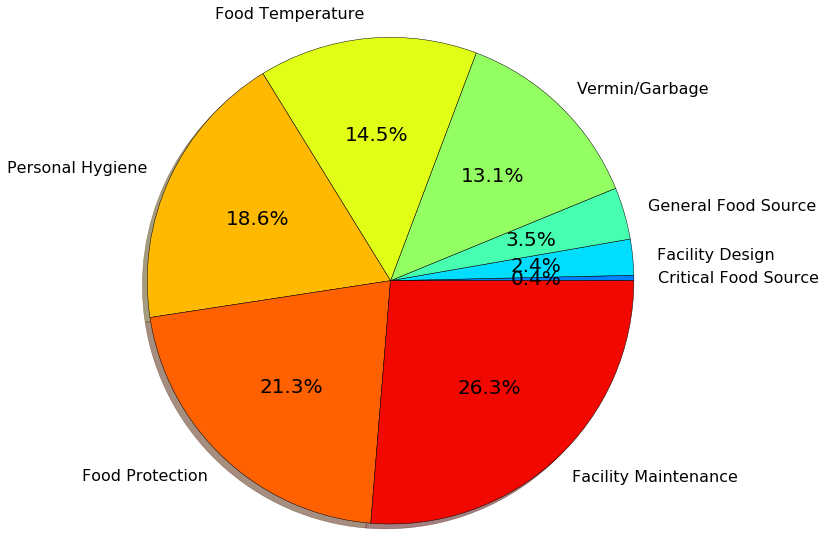
\includegraphics[scale = 0.5]{Figures/viol_group_pie.png}
\caption{Breakdown of Frequencies of Violation Groups}
\label{task_pie}
\end{figure}

\begin{sidewaystable}[]
\scalebox{0.7}{
\begin{tabular}{lcccccccc} \hline
 & (1) & (2) & (3) & (4) & (5) & (6) & (7) & (8) \\
VARIABLES & Facility Maintenance & Food Protection & Personal Hygiene & Food Temperature & Vermin/Garbage & Gen. Food Source & Facility Design & Crit. Food Source \\ \hline
 &  &  &  &  &  &  &  &  \\
Facility Maintenance & \cfbox{red}{1.012***} & -0.0212 & 0.0411*** & 0.00688 & 0.00619 & 0.000455 & -0.0111 & 0.00262 \\
 & (0.0193) & (0.0202) & (0.0143) & (0.0151) & (0.0213) & (0.0117) & (0.0103) & (0.00166) \\
Food Protection & -0.0597 & \cfbox{red}{0.940***} & 0.0543 & 0.234*** & 0.0642 & 0.0196 & -0.0107 & 0.00770 \\
 & (0.0637) & (0.0557) & (0.0494) & (0.0600) & (0.0629) & (0.0386) & (0.0295) & (0.00536) \\
Personal Hygiene & 0.0581*** & 0.0394** & \cfbox{red}{0.965***} & 0.0898*** & 0.0651*** & 0.0439*** & 0.0326*** & 0.00183 \\
 & (0.0170) & (0.0187) & (0.0146) & (0.0198) & (0.0195) & (0.0133) & (0.00927) & (0.00211) \\
Food Temperature & 0.0310 & 0.113*** & 0.0177 & \cfbox{red}{0.906***} & 0.0999*** & 0.0369*** & 0.0442*** & 0.00192 \\
 & (0.0202) & (0.0240) & (0.0167) & (0.0222) & (0.0246) & (0.0134) & (0.00993) & (0.00156) \\
Vermin/Garbage & 0.0449 & 0.0280 & -0.0909** & \cfbox{blue}{-0.178***} & \cfbox{red}{0.908***} & -0.0261 & 0.0158 & -0.00511 \\
 & (0.0540) & (0.0465) & (0.0442) & (0.0564) & (0.0520) & (0.0346) & (0.0253) & (0.00504) \\
Gen. Food Source & -0.0560* & -0.0629* & 0.00496 & -0.0256 & -0.0760** & \cfbox{red}{0.947***} & -0.0262 & -0.000915 \\
 & (0.0317) & (0.0353) & (0.0286) & (0.0281) & (0.0350) & (0.0241) & (0.0159) & (0.00359) \\
Facility Design & \cfbox{blue}{-0.184***} & \cfbox{blue}{-0.337***} & 0.0223 & 0.00730 & \cfbox{blue}{-0.400***} & \cfbox{blue}{-0.168***} & \cfbox{red}{0.791***} & -0.00582 \\
 & (0.0631) & (0.0824) & (0.0515) & (0.0731) & (0.0739) & (0.0408) & (0.0457) & (0.00844) \\
Crit. Food Source & -0.130 & -0.132 & -0.199 & -0.111 & 0.0138 & -0.265 & -0.0209 & \cfbox{red}{0.891***} \\
 & (0.204) & (0.237) & (0.151) & (0.213) & (0.229) & (0.173) & (0.114) & (0.0334) \\
 &  &  &  &  &  &  &  &  \\
Observations & 337,615 & 337,615 & 337,615 & 337,615 & 337,615 & 337,615 & 337,615 & 337,615 \\
 Time FE & YES & YES & YES & YES & YES & YES & YES & YES \\ \hline
\multicolumn{9}{c}{ Robust standard errors in parentheses} \\
\multicolumn{9}{c}{ *** p$<$0.01, ** p$<$0.05, * p$<$0.1} \\
\end{tabular}}
\footnotetext{Standard errors are two-way clustered at zipcode and inspector levels}
\caption{}
\label{multi_first_reg}
\end{sidewaystable}

\begin{sidewaystable}[h!]
\centering
\scalebox{0.7}{
\begin{tabular}{lcccccccc} \hline
 & (1) & (2) & (3) & (4) & (5) & (6) & (7) & (8) \\
VARIABLES & Facility Maintenance & Food Protection & Personal Hygiene & Food Temperature & Vermin/Garbage & Gen. Food Source & Facility Design & Crit. Food Source \\ \hline
 &  &  &  &  &  &  &  &  \\
Facility Maintenance & \textcolor{red}{-0.236***} & 0.00733 & 0.000184 & -0.00506 & -0.000922 & -0.00159 & 0.000981 & -0.000509 \\
 & (0.00961) & (0.0119) & (0.0107) & (0.00944) & (0.00766) & (0.00380) & (0.00295) & (0.00140) \\
Food Protection & \textcolor{blue}{-0.0776**} & \textcolor{red}{-0.177***} & -0.00731 & -0.0142 & \textcolor{blue}{-0.0397*} & -0.0100 & 0.00372 & \textcolor{brown}{0.00780*} \\
 & (0.0378) & (0.0306) & (0.0410) & (0.0253) & (0.0227) & (0.0113) & (0.0108) & (0.00400) \\
Personal Hygiene & 0.0222 & -0.00484 & \textcolor{red}{-0.189***} & -0.00771 & -0.000551 & 0.00458 & 0.00129 & 0.00217 \\
 & (0.0156) & (0.0103) & (0.0148) & (0.00957) & (0.00892) & (0.00489) & (0.00320) & (0.00173) \\
Food Temperature & 0.0148 & -0.0261 & 0.0133 & \textcolor{red}{-0.214***} & -0.00923 & 0.00613 & -0.00622 & -0.00153 \\
 & (0.0216) & (0.0163) & (0.0162) & (0.0134) & (0.0128) & (0.00722) & (0.00573) & (0.00243) \\
Vermin/Garbage & \textcolor{brown}{0.132***} & \textcolor{blue}{-0.0784*} & 0.00134 & 0.0446 & \textcolor{red}{-0.174***} & 0.0128 & -0.0105 & -0.00126 \\
 & (0.0439) & (0.0404) & (0.0544) & (0.0318) & (0.0283) & (0.0159) & (0.0138) & (0.00404) \\
Gen. Food Source & -0.0114 & -0.00139 & -0.0456 & -0.0103 & \textcolor{blue}{-0.0395*} & \textcolor{red}{-0.191***} & -0.0147 & -0.000895 \\
 & (0.0291) & (0.0348) & (0.0374) & (0.0334) & (0.0202) & (0.0199) & (0.00933) & (0.00395) \\
Facility Design & 0.0265 & \textcolor{blue}{-0.195**} & -0.00742 & 0.0168 & -0.0235 & 0.00421 & \textcolor{red}{-0.199***} & \textcolor{brown}{0.0169*} \\
 & (0.0787) & (0.0925) & (0.0776) & (0.0551) & (0.0612) & (0.0296) & (0.0239) & (0.00977) \\
Crit. Food Source & 0.274 & -0.284 & 0.279 & 0.125 & -0.0346 & -0.0233 & -0.0643 & \textcolor{red}{-0.185***} \\
 & (0.248) & (0.207) & (0.244) & (0.195) & (0.142) & (0.0848) & (0.0682) & (0.0298) \\
Observations & 149,831 & 149,829 & 149,831 & 149,829 & 149,829 & 149,831 & 149,829 & 149,831 \\
Dependent mean & 0.989 & 0.802 & 0.842 & 0.645 & 0.503 & 0.125 & 0.0694 & 0.0126 \\ \hline
\multicolumn{9}{c}{ Robust standard errors in parentheses} \\
\multicolumn{9}{c}{ *** p$<$0.01, ** p$<$0.05, * p$<$0.1} \\
\end{tabular}
}
\caption{}
\label{multi_second_reg}
\footnotetext{Standard errors are two-way clustered at zipcode and inspector levels.}
\end{sidewaystable}

%%%%%%%%%%%%%%%%%%%%%%%%%%%%%%%%%%%%%%%%%%%%%%
\iffalse
\begin{sidewaystable}[]
    \centering
    \scalebox{0.7}{
\begin{tabular}{lcccccccc} \hline
 & (1) & (2) & (3) & (4) & (5) & (6) & (7) & (8) \\
VARIABLES & Facility Maintenance & Food Protection & Personal Hygiene & Food Temperature & Vermin/Garbage & Gen. Food Source & Facility Design & Crit. Food Source \\ \hline
 &  &  &  &  &  &  &  &  \\
Facility Maintenance & \cfbox{red}{-0.0299**} & -0.0304** & -0.0131 & -0.0372** & -0.0437** & -0.00911 & -0.00103 & 0.00330 \\
 & (0.0134) & (0.0142) & (0.0148) & (0.0148) & (0.0184) & (0.00866) & (0.00569) & (0.00264) \\
Food Protection & 0.0134 & \cfbox{red}{-0.106**} & -0.0282 & -0.251*** & -0.155*** & -0.0612*** & 0.000699 & 0.0166* \\
 & (0.0398) & (0.0487) & (0.0466) & (0.0456) & (0.0567) & (0.0231) & (0.0259) & (0.00853) \\
Personal Hygiene & 0.0136 & -0.0767*** & \cfbox{red}{-0.0583***} & -0.106*** & -0.0804*** & -0.0219** & -0.00694 & 0.00373 \\
 & (0.0160) & (0.0177) & (0.0190) & (0.0185) & (0.0210) & (0.00967) & (0.00697) & (0.00372) \\
Food Temperature & -0.0215 & -0.122*** & -0.0202 & \cfbox{red}{-0.0869***} & -0.108*** & -0.00905 & -0.0246*** & -0.00258 \\
 & (0.0185) & (0.0198) & (0.0163) & (0.0200) & (0.0222) & (0.0131) & (0.00894) & (0.00437) \\
Vermin/Garbage & -0.00984 & -0.0749** & -0.0152 & 0.0950*** & \cfbox{red}{-0.0675*} & 0.0262 & -0.0221 & -0.00139 \\
 & (0.0292) & (0.0307) & (0.0367) & (0.0337) & (0.0388) & (0.0168) & (0.0203) & (0.00550) \\
Gen. Food Source & -0.0120 & -0.0154 & -0.0410* & -0.0359 & -0.0459* & \cfbox{red}{-0.0227} & -0.0222** & 0.000948 \\
 & (0.0173) & (0.0236) & (0.0214) & (0.0235) & (0.0262) & (0.0147) & (0.00881) & (0.00399) \\
Facility Design & -0.0241 & -0.137*** & -0.0732 & -0.0378 & -0.152*** & 0.0154 & \cfbox{red}{-0.0247} & 0.0205** \\
 & (0.0365) & (0.0473) & (0.0505) & (0.0452) & (0.0526) & (0.0248) & (0.0236) & (0.00838) \\
Crit. Food Source & -0.0391 & -0.258** & 0.102 & -0.114 & -0.0939 & 0.00645 & 0.00234 & \cfbox{red}{-0.0492*} \\
 & (0.136) & (0.131) & (0.125) & (0.150) & (0.136) & (0.0698) & (0.0703) & (0.0258) \\
 &  &  &  &  &  &  &  &  \\
 Observations & 156,317 & 156,316 & 156,316 & 156,317 & 156,317 & 156,316 & 156,316 & 156,316 \\ \hline
\multicolumn{9}{c}{ Robust standard errors in parentheses} \\
\multicolumn{9}{c}{ *** p$<$0.01, ** p$<$0.05, * p$<$0.1} \\
\end{tabular}   
}
\caption{}
\footnotetext{Standard errors are two-way clustered at zipcode and inspector levels}
\end{sidewaystable}
\fi
%%%%%%%%%%%%%%%%%%%%%%%%%%%%%%%%%%%%%%%%%%%%%%

\begin{table}[!htbp]
\centering
\scalebox{0.6}{\begin{tabular}{lcccccc} \hline
 & (1) & (2) & (3) & (4) & (5) & (6) \\
VARIABLES & Prob Call (OLS) & Prob Call (OLS) & Prob Call (OLS) & Prob Call (IV) & Prob Call (IV) & Prob Call (IV) \\ \hline
 &  &  &  &  &  &  \\
SCORE & -4.68e-05*** & -7.07e-06 & -9.04e-05*** & -8.93e-05* & -9.14e-05* & -6.12e-05 \\
 & (1.54e-05) & (1.57e-05) & (1.79e-05) & (4.76e-05) & (4.98e-05) & (6.16e-05) \\
Months Since Inspection &  & 0.000540*** & -1.94e-05 &  & 0.000498*** & 0.000739* \\
 &  & (3.73e-05) & (6.63e-05) &  & (4.33e-05) & (0.000434) \\
c.mon\_from\_inspect\#c.SCORE &  &  & 5.03e-05*** &  &  & -2.19e-05 \\
 &  &  & (5.81e-06) &  &  & (3.96e-05) \\
 &  &  &  &  &  &  \\
Observations & 1,223,207 & 1,223,207 & 1,223,207 & 1,223,207 & 1,223,207 & 1,223,207 \\
Year-Month FE & YES & YES & YES & YES & YES & YES \\
Restaurant FE & YES & YES & YES & YES & YES & YES \\
 Dependent Mean & 0.0145 & 0.0145 & 0.0145 & 0.0145 & 0.0145 & 0.0145 \\ \hline
\multicolumn{7}{c}{ Robust standard errors in parentheses} \\
\multicolumn{7}{c}{ *** p$<$0.01, ** p$<$0.05, * p$<$0.1} \\
\end{tabular}
}
\caption{Impact of Inspection Scores on the Probability of Receiving 311 Complaint Call}
\label{calls}
\footnotetext{Sample include inspections conducted by inspectors who have conducted at least 50 inspections of the same type. The dependent variable is an indicator variable for whether a restaurant receives at least one complaint call in a month. Standard errors are two-way clustered at zipcode and inspector levels.}
\label{complaint_table}
\end{table}

\end{document}

